\documentclass[11pt,a4paper]{ctexart}

\usepackage[margin=2.6cm]{geometry}
\usepackage{amsmath,amssymb,amsthm}
\usepackage{graphicx}
\usepackage{booktabs}
\usepackage{hyperref}
\usepackage{xcolor}
\usepackage{listings}
\usepackage{caption}

\graphicspath{{figures/}}
\hypersetup{colorlinks=true, linkcolor=blue!50!black, urlcolor=blue!60!black}
\lstset{
  basicstyle=\ttfamily\small,
  breaklines=true,
  frame=single,
  columns=fullflexible,
  backgroundcolor=\color{gray!7}
}

\newtheorem{definition}{定义}[section]
\newtheorem{theorem}{定理}[section]
\newtheorem{lemma}{引理}[section]
\newtheorem{proposition}{命题}[section]
\newtheorem{example}{例}[section]

\title{第 8 章 \quad Estimation of the mean and covariance / 均值与协方差估计}
\author{基于 \textit{A Course in Time Series Analysis} 的中文讲义与 Python 实践}
\date{}

\begin{document}
\maketitle

\section*{本章学习目标}

本章按照原文 \textit{Estimation of the mean and covariance} 的小节顺序整理，保留主要定义、定理、模型公式和练习方向，并将原文中的 R 实践思路改写为 Python 工程实践。

完成本章后，应能够：
\begin{itemize}
  \item 推导相关序列下样本均值的抽样性质；
  \item 定义样本自协方差和样本自相关；
  \item 理解自相关检验、Portmanteau 检验及稳健版本；
  \item 掌握 Newey-West/HAC 长期方差估计；
  \item 区分长记忆和均值结构变化。
\end{itemize}

\section{均值估计}

样本均值仍定义为
\[
  \bar X_n=\frac1n\sum_{t=1}^n X_t.
\]
若 \(\{X_t\}\) 为平稳线性过程且协方差绝对可和，则
\[
  \sqrt n(\bar X_n-\mu)\Rightarrow N(0,\sigma_L^2),
\qquad
  \sigma_L^2=\sum_{k=-\infty}^{\infty}c(k).
\]
\begin{theorem}[样本均值的渐近性质，原文 Theorem 8.1.1]
在线性时间序列和适当矩条件下，样本均值相合且渐近正态；渐近方差为长期方差，而不是单期方差 \(c(0)\)。
\end{theorem}

\section{协方差估计}

经验自协方差定义为
\[
  \hat c(h)=\frac1n\sum_{t=1}^{n-h}(X_t-\bar X)(X_{t+h}-\bar X),
\]
样本 ACF 为 \(\hat\rho(h)=\hat c(h)/\hat c(0)\)。

\begin{lemma}[经验协方差，原文 Lemma 8.2.1]
若均值已知或由样本均值替代，在平稳和矩条件下，\(\hat c(h)\) 是 \(c(h)\) 的相合估计。
\end{lemma}

\begin{theorem}[样本自协方差渐近分布，原文 Theorem 8.2.1--8.2.3]
对满足短记忆和四阶矩条件的线性序列，有限个样本自协方差组成的向量渐近正态，其协方差由二阶和四阶累积量决定。
\end{theorem}

\section{相关性检查}

白噪声检验常基于若干阶样本自相关。Box-Pierce/Ljung-Box 型统计量形如
\[
  Q_m=n\sum_{h=1}^m\hat\rho(h)^2
\]
或带有限样本修正。若序列为白噪声，\(Q_m\) 近似服从 \(\chi_m^2\)。

\subsection{稳健 Portmanteau 检验}

当存在条件异方差或更一般弱依赖时，普通 Portmanteau 检验的方差估计可能失真。稳健版本用 HAC 型协方差替代简单方差，以保持检验大小。

\section{偏相关检查}

样本 PACF 用于识别 AR 阶数。若真实模型为 AR(p)，则 p 阶之后的理论 PACF 为 0；样本 PACF 可用近似置信带判断是否显著。

\section{Newey-West 估计与拟合优度}

长期方差
\[
  \sigma_L^2=\sum_{k=-\infty}^{\infty}c(k)
\]
可用截断加权估计：
\[
  \hat\sigma_L^2=\hat c(0)+2\sum_{k=1}^{m}w_k\hat c(k),
\]
其中 Bartlett 权重为
\[
  w_k=1-\frac{k}{m+1}.
\]
这就是 Newey-West/HAC 估计的核心形式。

拟合优度检查通常对模型残差作 ACF、PACF 和 Portmanteau 检验。如果模型捕捉了线性依赖，残差应接近白噪声。

\section{长记忆与结构变化}

原文提醒：样本 ACF 缓慢衰减可能来自长记忆，也可能来自均值变化或趋势未处理。二者在图形上相似，但统计含义不同，需要结合趋势建模、分段分析和频域诊断判断。

\section{原文定理与练习补充}

\subsection{8.2.1 自协方差估计渐近性质}
\begin{theorem}[原文 Theorem 8.2.1]
若 \(\{X_t\}\) 为均值为 0 的线性平稳过程并满足矩条件，则固定滞后 \(h\) 的样本自协方差 \(\hat c(h)\) 相合，并具有渐近正态性质。
\end{theorem}

\subsection{8.2.2 样本自相关渐近性质}
\begin{theorem}[原文 Theorem 8.2.2--8.2.3]
样本自协方差和样本自相关组成的有限维向量在短记忆条件下渐近正态。该结果支撑 ACF 图置信带和相关性检验。
\end{theorem}

\subsection{8.2.3 样本自协方差之间的协方差}
\begin{example}[原文 Example 8.2.1]
对因果 AR(1) 模型 \(X_t=\phi X_{t-1}+\varepsilon_t\)，可显式计算样本自协方差极限协方差，用来说明不同滞后估计量之间并非独立。
\end{example}

\subsection{8.6 与 8.7}
第 8.6 节讨论模型拟合优度，第 8.7 节区分长记忆和均值变化。Exercise 8.1--8.3 研究 iid、MA(1) 和 block bootstrap；Exercise 8.4 检查偏相关。

\begin{lemma}[原文 Lemma 8.2.2]
在 Theorem 8.2.2 条件下，样本自相关可由样本自协方差通过 Delta 方法得到渐近分布。
\end{lemma}

\section{Python 工程实践}

在本章目录下运行：
\begin{lstlisting}[language=bash]
python scripts/ch08_generate_figures.py
\end{lstlisting}

脚本会把图像写入本章 \texttt{figures/} 目录。当前图像用于配合本章核心概念的仿真说明；若后续补齐原始数据文件，可把模拟数据替换为原文真实数据案例。

\begin{figure}[htbp]
  \centering
  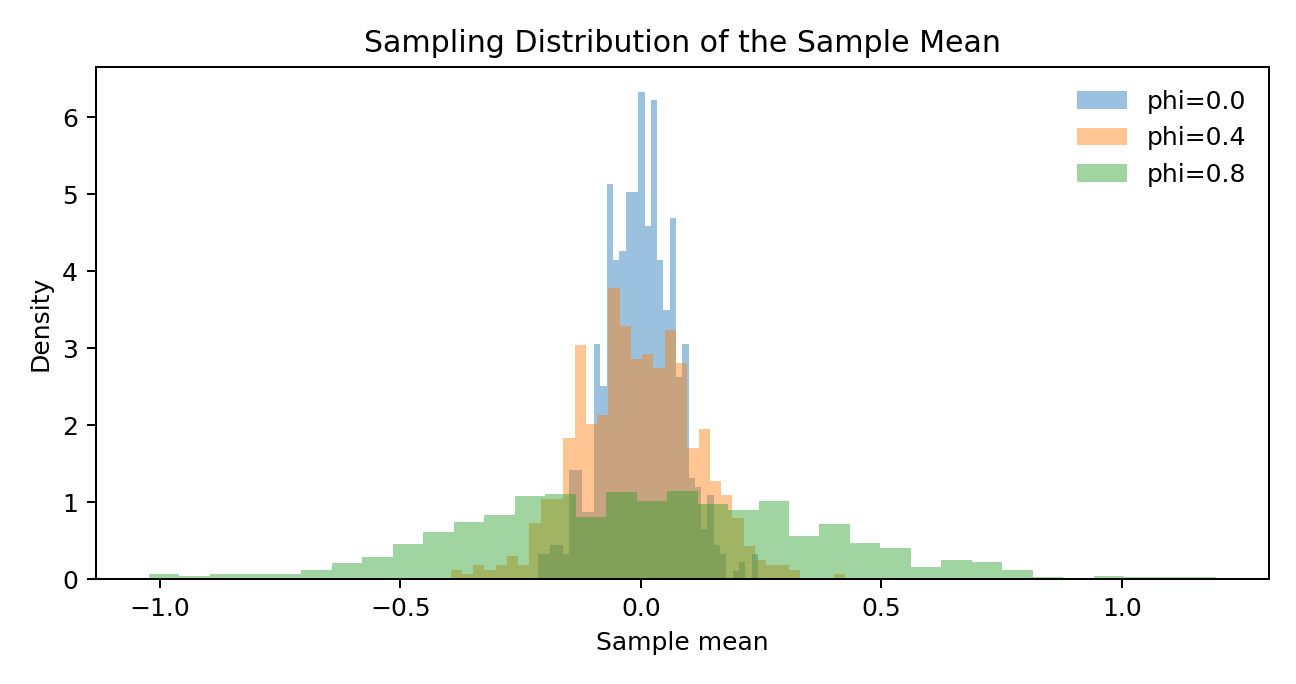
\includegraphics[width=0.86\textwidth]{ch08_fig01_sample_mean_dependence.png}
  \caption{不同相关强度下样本均值的抽样分布：相关性越强，有效样本量越小。}
\end{figure}

\begin{figure}[htbp]
  \centering
  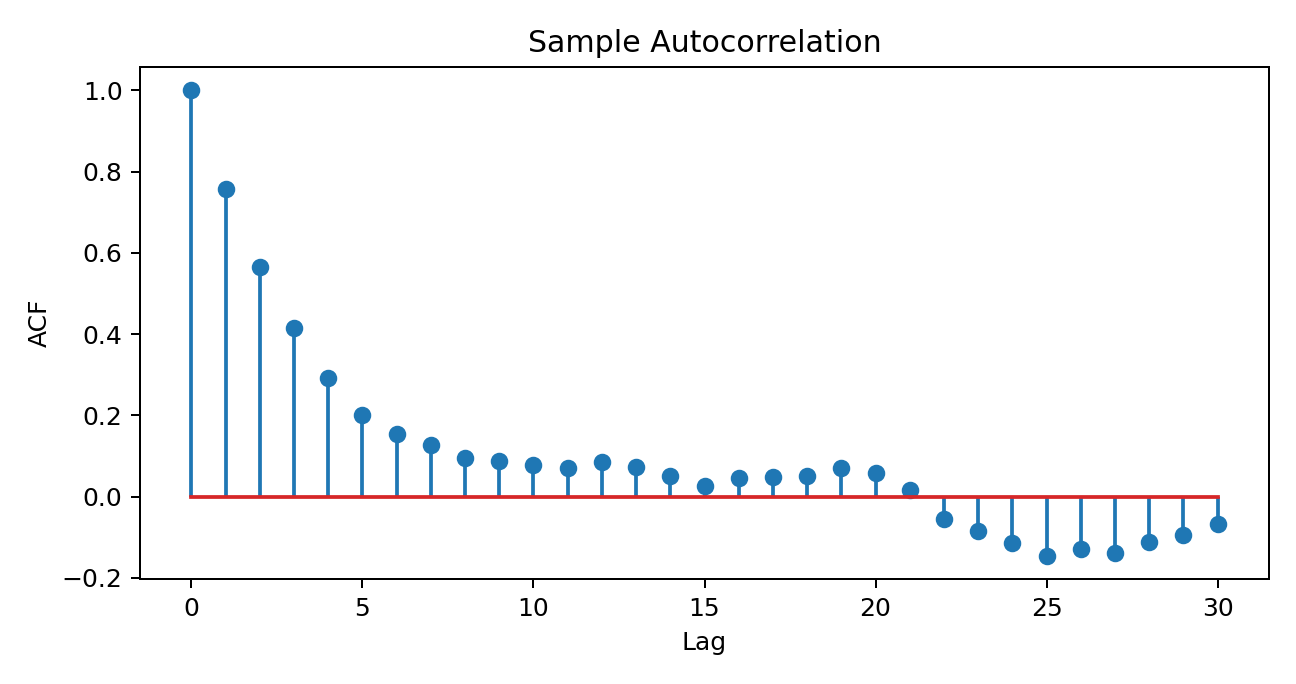
\includegraphics[width=0.86\textwidth]{ch08_fig02_sample_acf.png}
  \caption{样本 ACF 示例：估计序列在不同滞后上的线性依赖。}
\end{figure}

\section{练习提要}

原文练习主要围绕下列方向展开：
\begin{itemize}
  \item 在 iid、MA(1)、AR(1) 条件下推导样本自协方差的方差；
  \item 用 block bootstrap 估计样本均值的有限样本分布；
  \item 实现 Portmanteau 检验和稳健版本；
  \item 计算 Newey-West 标准误并比较普通标准误。
\end{itemize}

\section*{本章小结}

第 8 章把平稳理论转化为可计算估计量。均值、协方差、ACF、PACF 和长期方差估计是时间序列实证分析的基本工具，其中关键始终是正确处理相关性。

\end{document}
